\documentclass[11pt,a4paper]{article}
\usepackage[utf8]{inputenc}
\usepackage[german]{babel}
\usepackage[T1]{fontenc}
\usepackage{amsmath}
\usepackage{amsfonts}
\usepackage{amssymb}
\usepackage{graphicx}
\usepackage[margin=1.25cm]{geometry} % Puts the same margin on all borders of the document

% Packages

\usepackage{hyperref} % Generate hyperlinks to referenced items
\usepackage{adjustbox} % Used to change parameters in \includegraphics[scale=•]{•}
\usepackage{enumitem} % Provides several options for lists
\usepackage{verbatim} % Package to use \begin{comment}
\usepackage{pdfpages} % Used to import PDF pages
\usepackage{multirow} % Allows us to have a single cell in a table span multiple rows
\usepackage{makecell} % Allows us to format multiple lines in a single cell
\usepackage{minted} % Used to syntax highlight code
\usepackage{xcolor}  % Gives access to coloring text
\usepackage{longtable} % Allows us to create a table over multiple pages
\usepackage{float} % Improved placement of floating items
\usepackage{pdfpages} % Used to import pdf pages
\usepackage{booktabs} % Used for horizontal lines instead of \hline



% Settings

\graphicspath{{./files/}} % Sets path for files to the files folder in the same directory

\hypersetup{
    colorlinks=false, %set true if you want colored links
    linktoc=all,     %set to all if you want both sections and subsections linked
    linkcolor=blue,  %choose some color if you want links to stand out
}

\tcbuselibrary{minted,skins}

\definecolor{vlcodebg}{rgb}{0.85,0.85,0.85}

% Kudos an Rubos
% code environment with boxes
\newtcblisting{ccode}[2][]{
    listing engine=minted,
    colback=vlcodebg!30, 
    colframe=black!70,
    listing only,
    %minted style=colorful,
    minted language=c,
    minted options={ 
      linenos=true,
      numbersep=3mm,
      texcl=true,
      #1 
      },
      left=5mm,
      enhanced,
      overlay={
                \begin{tcbclipinterior}
                  \fill[black!25] (frame.south west) rectangle ([xshift=5mm]frame.north west); % Zeilennummernbereich färben
                \end{tcbclipinterior}
              },
      #2
}

\begin{document}

\begin{center}
    {\huge \textbf{AUD Klausurblatt SoSe 2020 | Janson/Fischlin}}
\end{center}

\section*{Definitionen/Wissen}
\subsection*{Sortier-Algorithmen in einem Satz}
\begin{itemize}
    \item \textit{InsertionSort}: Sortierthalten der linken Teilfolge, neuen Wert an richtige Position einfügen
    \item \textit{BubbleSort}: Vergleiche Paare von benachbarten Schlüsselwerten
    \item \textit{SelectionSort}: Wähle kleinstes Element und tausche es nach vorne
    \item \textit{MergeSort}: Teilen, sortiertes Zurückschreiben in Array
    \item \textit{QuickSort}: Vergleich der Werte mithilfe PivotElement, rekursiver Aufruf auf Teilarray
\end{itemize}

\subsection*{Asymptotik}
\begin{itemize}
    \item $\frac{f(n)}{g(n)} = 0$ $\Rightarrow$ $f(n) = o(g(n))$
    \item $\frac{f(n)}{g(n)}: konvergent$ $\Rightarrow$ $f(n) = O(g(n))$
    \item $o(n) \in O(n)$ $\Rightarrow$ schließt alle anderen aus
    \item $f(n) = g(n)$ $\Rightarrow$ $f(n) = \Theta(g(n))$
\end{itemize}

\subsection*{Master-Theorem}
\begin{itemize}
    \item \textit{Anwendbar?}
        \begin{itemize}
            \item $a \geq 1$ und konstant?
            \item $b > 1$ und konstant?
            \item $f(n)$ positiv?
        \end{itemize}
    \item \textit{Vorgehen}
        \begin{itemize}
            \item Berechnung von $log_b(a)$
            \item Vergleich mit $f(n)$
                \begin{itemize}
                    \item {\makebox[8cm][l]{$f(n)$ \textbf{polynomial kleiner} als $n^{log_b(a)}$}}  $\Rightarrow$ $T(n) = \Theta(n^{log_b(a)})$
                    \item[] $(f(n) = O(n^{log_b(a-\epsilon)})$, $\epsilon > 0$)
                    \item {\makebox[8cm][l]{$f(n)$ und $n^{log_b(a)}$ \textbf{gleiche Größe}}}  $\Rightarrow$ $T(n) = \Theta(n^{log_b(a)} lg(n))$
                    \item[] $(f(n) = \Theta(n^{log_b(a)})$
                    \item {\makebox[8cm][l]{$f(n)$ \textbf{polynomial größer} als $n^{log_b(a)}$ und}} 
                    \item[] {\makebox[8cm][l]{$af(\frac{n}{b}) \leq c~f(n)$, ($\epsilon < 1)$}}  $\Rightarrow$ $T(n) = \Theta(f(n))$
                    \item[] ($f(n) = \Omega (n^{log_b(a + \epsilon)})$, $\epsilon > 0$) 
                \end{itemize}
        \end{itemize}
\end{itemize}

\subsection*{String-Matching}
\subsubsection*{Allgemein}
    \begin{itemize}
        \item {\makebox[4cm][l]{durchsuchender Text:}}  Array \texttt{T} der Länge \texttt{lenTxt}
        \item {\makebox[4cm][l]{Textmuster:}}  Array \texttt{P} der Länge \texttt{lenPat $\leq$ lenTxt}
        \item {\makebox[4cm][l]{Gesucht:}}  alle gültigen Verschiebungen mit denen \texttt{P} in \texttt{T} auftaucht
        \item {\makebox[4cm][l]{Rückgabe:}} alle \texttt{sft $\in \mathbb{N}$}, sodass \texttt{T[sft,$\dots$,sft+lenPat-1] = P} gilt
    \end{itemize}

\subsubsection*{NaiveStringMatching}
\begin{minipage}{0.45\textwidth}
    \textit{Pseudocode:}
    \begin{ccode}[autogobble,escapeinside=||]{title={NaiveStringMatching(T,P)}}
    lenTxt = length(T)
    lenPat = length(P)
    L = empty
    FOR sft = 0 TO lenTxt - lenPat DO
        isValid = TRUE
        FOR j = 0 TO lenPat - 1 DO
            IF P[j] |$\neq$| T[sft+j] THEN
                isValid = FALSE
        IF isValid THEN
            L = append(L, sft)
    RETURN L
    \end{ccode}
\end{minipage}
\begin{minipage}{0.5\textwidth}
    \textit{Beispiel:} \texttt{T=[h,e,h,e,h,h,h,e,y,h]}, \texttt{P=[h,e,h]} \\
    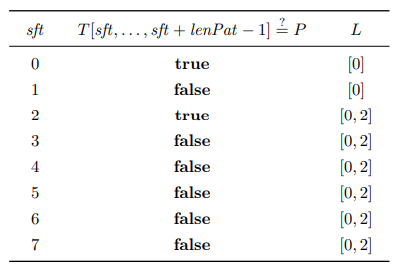
\includegraphics[height=6.5cm]{naiveStringMatchingBsp.png}
\end{minipage}

\subsection*{Queue mithilfe von zwei Stacks}

$enqueue$ pusht auf den ersten Stack. \\
$dequeue$ wird als $pop(S_2)$ definiert. \\
Falls der zweite Stack leer ist werden alle Elemente aus $S_1$ geholt und in $S_2$ überführt. \\
Dann wird das erste Element von $S_2$ ausgegeben. \\
\centerline{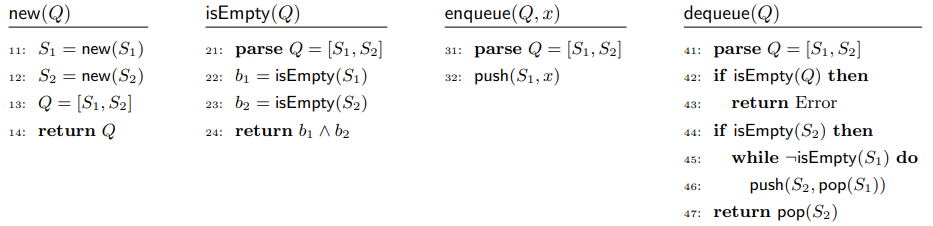
\includegraphics[width=12cm]{stackQueue.png}}

\subsection*{Stack mithilfe von zwei Queues}

Eine der beiden Queues bleibt immer leer (anfangs $Q_2$) \\
$push$ fügt Wert immer der leeren Queue hinzu. \\
$pop$ holt alle Elemente bis auf das letzte aus der Queue zurück und fügt sie in die leere ein. \\
Das letzte Element wird dann ausgegeben. \\
\centerline{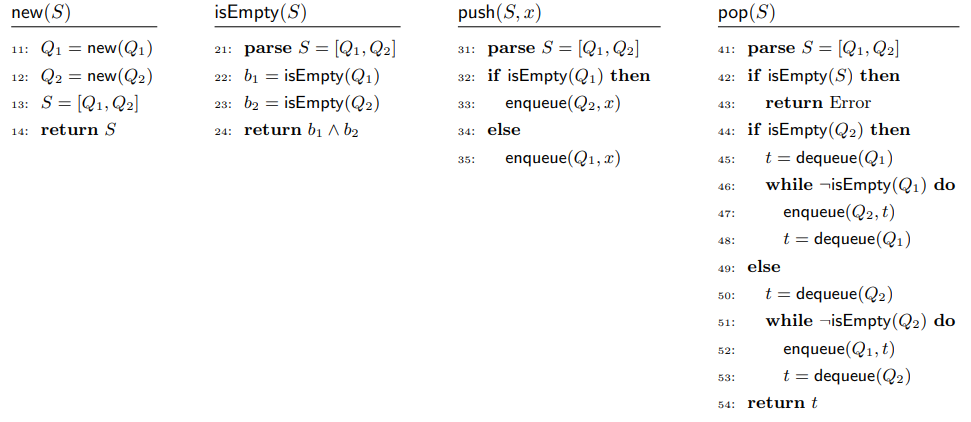
\includegraphics[width=12cm]{queueStack.png}}

\pagebreak

\section*{Baumoperationen}

\subsection*{BST}
\subsubsection*{Löschen}
\centerline{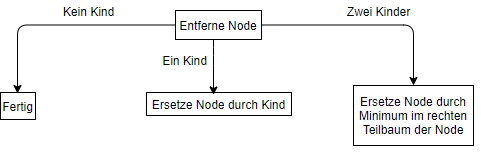
\includegraphics[width=10cm]{BSTDelete.png}}

\subsection*{RBT}
\subsubsection*{Insert}
\centerline{Wie im BST, neuen Knoten rot färben, danach FixUp:}
\centerline{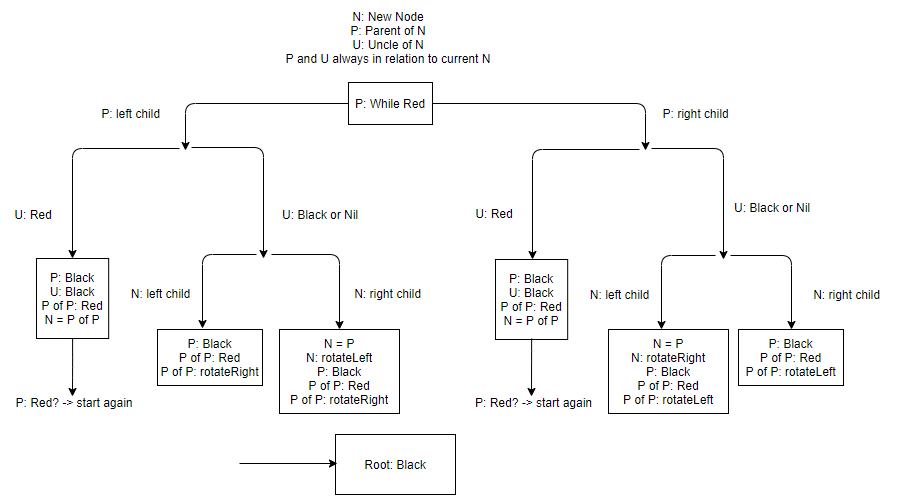
\includegraphics[width=15cm]{RBTInsert.png}}

\subsection*{AVL-Bäume}
\subsubsection*{Einfügen/Löschen}
\centerline{Einfügen und Löschen wie beim BST, danach jeweils Rebalancieren:}
\centerline{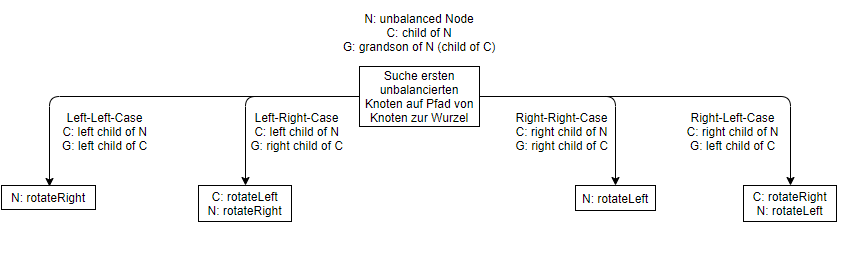
\includegraphics[width=15cm]{AVLRebalance.png}}
Beachte beim Löschen: 
    \begin{itemize}
        \item Wahl von C: größter Teilbaum von N (eindeutig, da N unbalanciert)
        \item Wahl von G: größter Teilbaum von C (nicht eindeutig, Wahl Rechts-Rechts/Links-Links)
        \item \textbf{Potenziell} müssen mehrere Knoten bearbeitet werden $\Rightarrow$ alle Knoten bis Wurzel prüfen
    \end{itemize}

\subsection*{Splay-Bäume}
\begin{itemize}
    \item Suchen: Spüle gesuchten Knoten an die Wurzel (alternativ zuletzt besuchten Knoten)
    \item Einfügen: Einfügen nach BST-Regeln und danach Hochspülen des Knotens
    \item Löschen:
        \begin{itemize}
            \item[1.] zu löschenden Knoten hochspülen
            \item[2.] Knoten löschen
            \item Falls nur ein Kind: Dieses Kind neue Wurzel und fertig
            \item {\makebox[3cm][l]{Falls zwei Kinder:}}  Spüle größten Knoten im linken Teilbaum hoch
            \item[] {\makebox[3cm][l]{}} Hänge danach beide Teilbäume an diesen Knoten
        \end{itemize}
\end{itemize}

\subsubsection*{Spülen}
\centerline{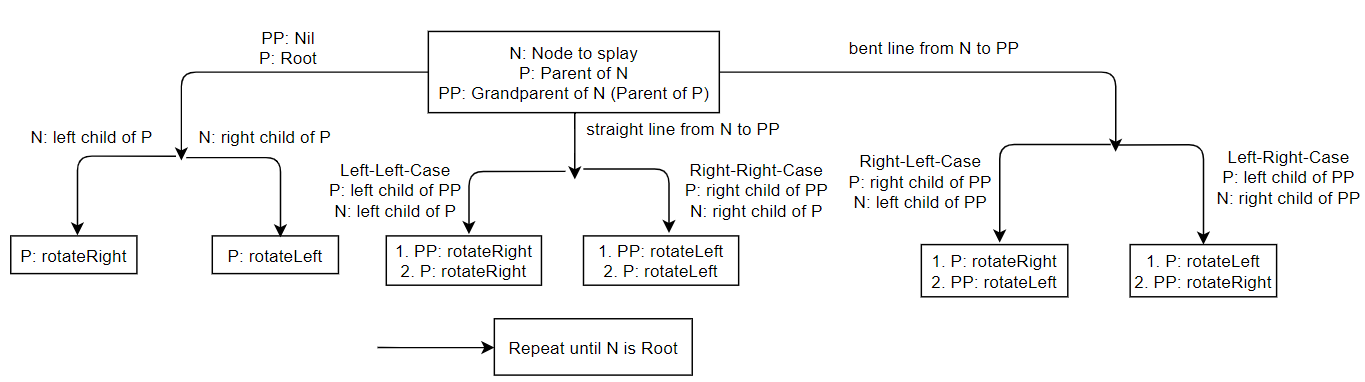
\includegraphics[width=15cm]{SplaySplay.png}}

\subsection*{Heaps}
\subsubsection*{Heap-Sort}
    \begin{enumerate}
        \item Array wird als Heap aufgefasst
        \item Heapeigenschaft wird wiederhergestellt (Heapify)
        \item Extrahieren der Wurzel (Maximum) und Ersetzen durch \string"letztes\string" Blatt
        \item Wieder Heapify um Wert an die richtige Stelle zu rücken
        \item Falls der Baum noch nicht leer ist, gehe zu Schritt 3
    \end{enumerate}

\noindent
Heapify: beginnend bei \texttt{ceil((H.length-1)/2) - 1} bis 0: vertausche nach unten, falls Parent kleiner als Child
\centerline{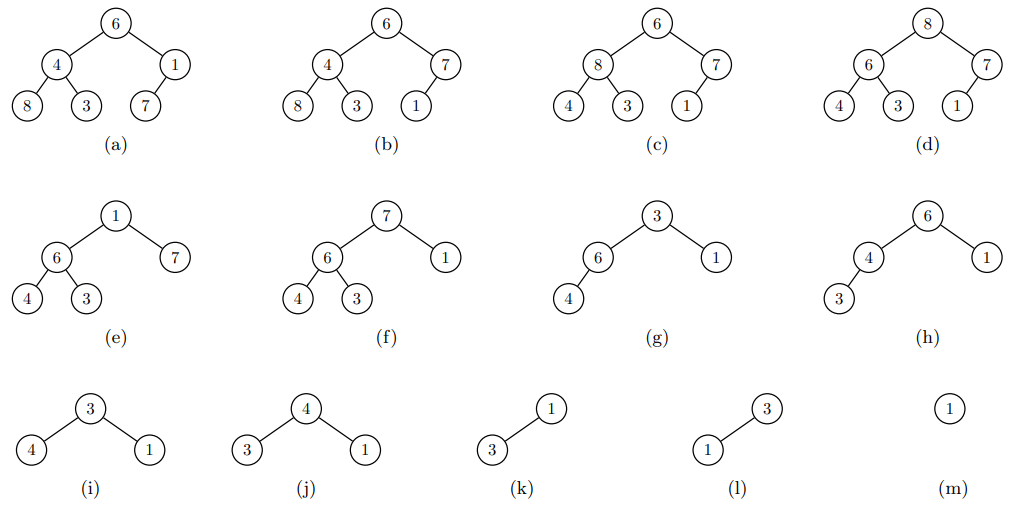
\includegraphics[width=15cm]{heapSortBsp.png}}

\subsection*{B-Bäume vom Grad \texttt{t}}
\centerline{Knoten zwischen \texttt{[t-1, $\dots$,2t-1]} Werte (Wurzel: \texttt{[1, $\dots$,2t-1])}} 
\subsubsection*{Einfügen}
\texttt{Split:}
    \begin{itemize}
        \item Aufbrechen der vollen (\texttt{2t-1}) Node
        \item Hinzufügen der mittleren Node zur Elternnode
        \item Aus den anderen Nodes entstehen nun jeweils einzelne Kinder
        \item Splitten an der Wurzel erzeugt neue Wurzel und erhöht Baumhöhe um 1
    \end{itemize}

\centerline{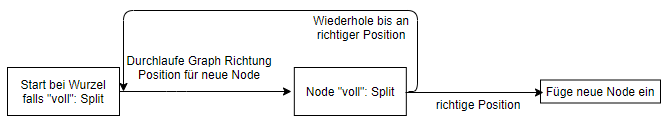
\includegraphics[width=15cm]{BInsert.png}}

\subsubsection*{Löschen}
\begin{enumerate}
    \item Start bei Wurzel
    \item[] Wurzel: \texttt{1} Wert | Kinder der Wurzel: \texttt{t-1} Werte $\rightarrow$ Verschmelze Kinder und Wurzel
    \item Durchlaufe Graph von Node bis zum löschenden Knoten
    \item Überprüfe bei jeder Node:
    \item[]
        \begin{minipage}{0.45\textwidth}
            \textit{Verschmelzen} \\
            Kind + Geschwister \texttt{t-1} Werte \\
            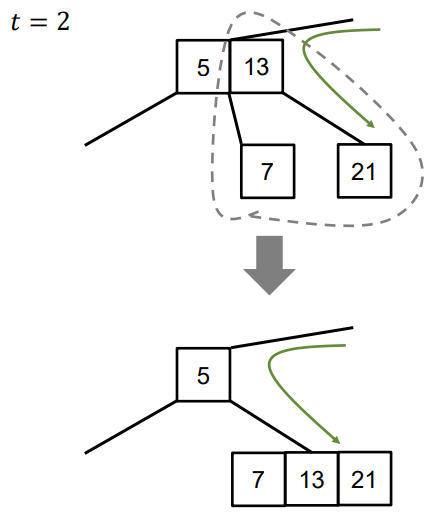
\includegraphics[width=5cm]{bbaumMelt.png}
        \end{minipage} 
        \begin{minipage}{0.45\textwidth}
        \textit{Rotation} \\
        Kind nur \texttt{t-1} Werte \\
        Geschwister jedoch mehr als \texttt{t-1} Werte \\
        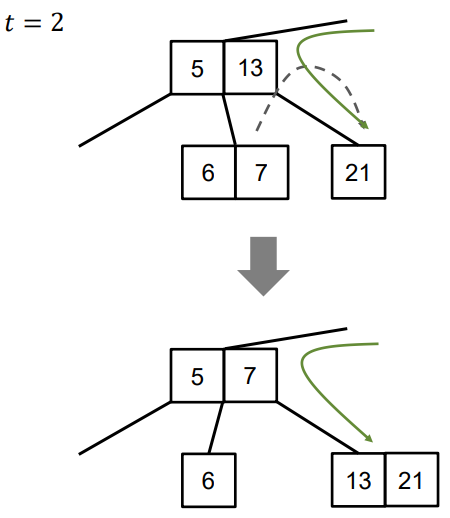
\includegraphics[width=5cm]{bbaumRot.png}
        \end{minipage}
    \item Knoten gefunden:
        \begin{itemize}
            \item \textbf{Löschen im Blatt:} Einfach entfernen, fertig
            \item \textbf{Löschen im inneren Knoten:}
            \item[]
                \begin{minipage}{0.4\textwidth}
                    \textit{Verschmelzen} \\
                    Beide Kinder \texttt{t-1} Werte \\
                    $\rightarrow$ Kindknoten verschmelzen \\
                    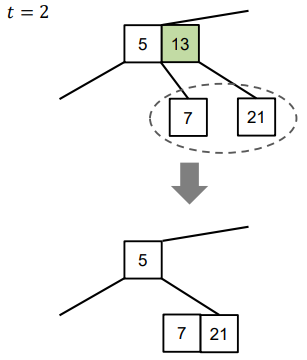
\includegraphics[width=5cm]{bbaumInnerMelt.png}
                \end{minipage} 
                \begin{minipage}{0.5\textwidth}
                \textit{Verschieben} \\
                Eines der Kinder mehr als \texttt{t-1} Werte \\
                Größten Wert vom linken Kind nach oben kopieren oder \\
                Kleinsten Wert vom rechten Kind nach oben kopieren\\
                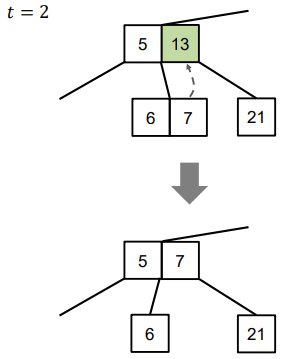
\includegraphics[width=5cm]{bbaumInnerRot.png}
                \end{minipage}
                \end{itemize}
\end{enumerate}



\pagebreak

\section*{Anwendungsbeispiel}

\subsection*{Sorting}

\subsubsection*{Insertion Sort}
\centerline{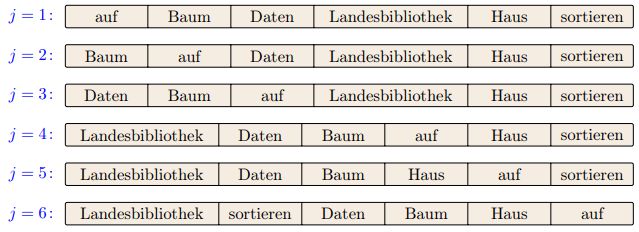
\includegraphics[width=12cm]{insertionSortBsp.png}}

\subsubsection*{Merge Sort}
\centerline{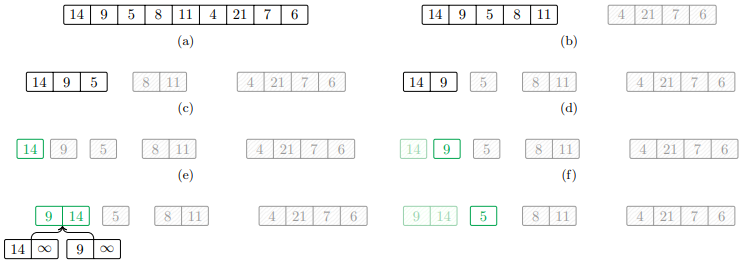
\includegraphics[width=12cm]{mergeSortBsp.png}}

\subsubsection*{Quick Sort}
\centerline{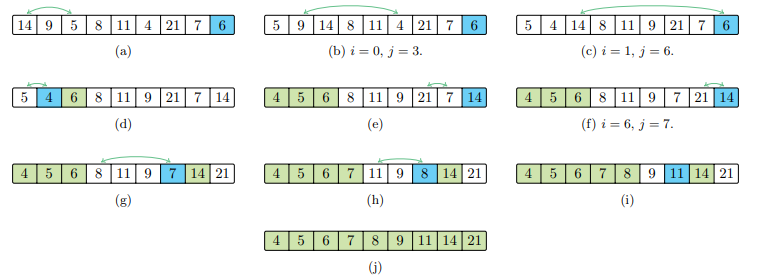
\includegraphics[width=12cm]{quickSortBsp.png}}

\subsection*{Basic Data Structures}

\subsubsection*{Stacks}
\centerline{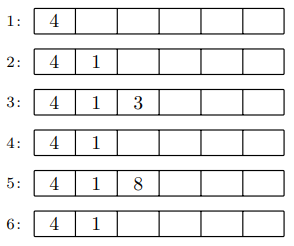
\includegraphics[width=5cm]{stackBsp.png}}

\subsubsection*{Queues}
\centerline{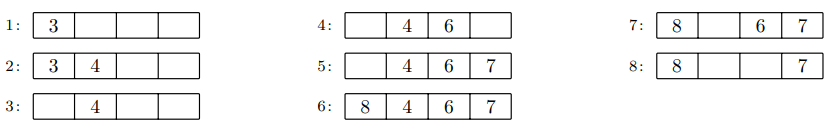
\includegraphics[width=12cm]{queueBsp.png}}

\section*{Pseudocode}
\subsection*{Sorting}
    \begin{ccode}[autogobble]{title=Insertion Sort(A)}  
        FOR j = 1 TO A.length - 1
          key = A[j]
          // Füge A[j] in die sortierte Sequenz A[0...j-1] ein
          i = j - 1
          WHILE i >= 0 and A[i] > key
              A[i + 1] = A[i]
              i = i - 1
          A[i + 1] = key
    \end{ccode}

    \begin{ccode}[autogobble]{title=BubbleSort(A)}  
        FOR i = 0 TO A.length - 2
            FOR j = A.length - 1 DOWNTO i + 1
                IF A[j] < A[j-1]
                    SWAP(A[j], A[j-1])
        \end{ccode}
    
        \begin{ccode}[autogobble]{title=SelectionSort(A)}
        FOR i = 0 TO A.length - 2
            k = i 
            FOR j = i + 1 TO A.length - 1
                IF A[j] < A[k]
                    k = j 
            SWAP(A[i], A[k])
        \end{ccode}
    
    \subsubsection*{Merge Sort}
        \begin{ccode}[autogobble,escapeinside=||]{title={MergeSort(A, p, r)}}
        IF p < r
            q = |$\left \lfloor \texttt{(p+r)/2} \right \rfloor$| // Teilen in 2 Teilfolgen 
            MERGE-SORT(A,p,q) // Sortieren der beiden Teilfolgen
            MERGE-SORT(A,q+1,r)
            MERGE(A,p,q,r) // Vereinigung der beiden sortierten Teilfolgen
        \end{ccode}
    
        \begin{ccode}[autogobble,escapeinside=||]{title={MERGE(A,p,q,r)}}
        // Geteiltes Array an Stelle q
        |$n_1$| = q - p + 1
        |$n_2$| = r - q 
        Let L[0...|$n_1$|] and R[0...|$n_2$|] be new arrays 
        FOR i = 0 TO |$n_1$| - 1 // Auffüllen der neu erstellten Arrays
            L[i] = A[p + i]
        FOR j = 0 TO |$n_2$| - 1
            R[j] = A[q + j + 1]
        L[|$n_1$|] = |$\infty$| // Einfügen des Sentinel-Wertes
        R[|$n_2$|] = |$\infty$|
        i = 0
        j = 0
        FOR k = p TO r  // Eintragweiser Vergleich der Elemente          
            IF L[i] |$\leq$| R[j]
                A[k] = L[i] // Sortiertes Zurückschreiben in Original-Array
                i = i + 1
            ELSE 
                A[k] = R[j]
                j = j + 1
        \end{ccode}
    
    \subsubsection*{Quicksort}
        \begin{ccode}[autogobble,escapeinside=||]{title={QUICKSORT(A,p,r)}}
        IF p < r    // Überprüfung, ob Teilarray leer ist
            q = PARTITION(A,p,r)
            QUICKSORT(A,p,q-1)
            QUICKSORT(A,q+1,r)
        \end{ccode}
    
        \begin{ccode}[autogobble,escapeinside=||]{title={PARTITION(A,p,r)}}
        x = A[r]    // Wahl des Pivotelements
        i = p - 1   // Index i setzen
        FOR j = p TO r - 1 // Auffüllen des Teilarrays mit Elementen
            IF A[j] |$\leq$| x
                i = i + 1
                SWAP(A[i], A[j]) /
        SWAP(A[i+1], A[r]) // Tausch des Pivotelements
        RETURN i + 1 // Neuer Index des Pivotelements
        \end{ccode}
    
\section*{MasterTheorem - Beispiele}

\centerline{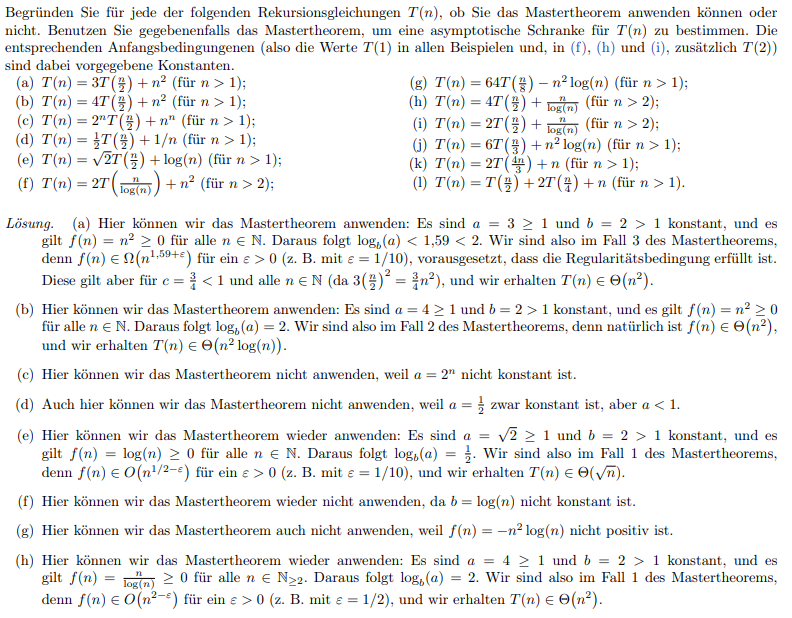
\includegraphics[width=15cm]{masterTheoremBsp1.png}}
\centerline{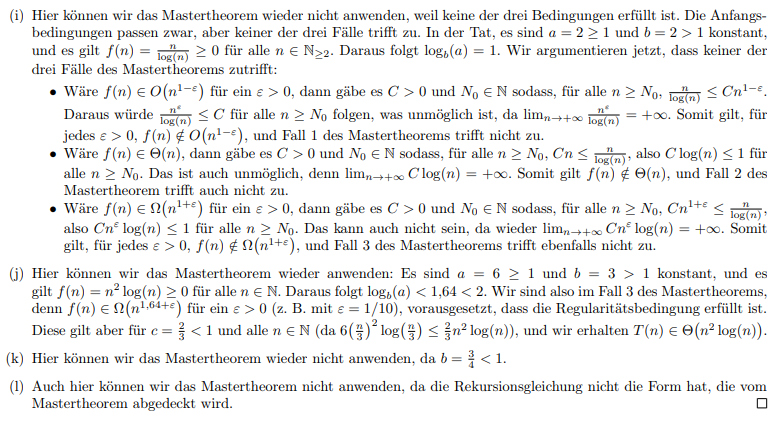
\includegraphics[width=15cm]{masterTheoremBsp2.png}}
    
\end{document}